\newpage
\chapter{Smart Grid: architettura, componenti ed evoluzione}

\section{Introduzione alle Smart Grid}



Una Smart Grid - Rete Intelligente - è l'evoluzione della tradizionale rete elettrica. Si basa su componenti avanzati di \textbf{rilevamento}, \textbf{comunicazione} e \textbf{decisione} per ottenere una trasmissione e distribuzione di energia \textbf{sicura}, \textbf{efficiente} e \textbf{resiliente}. \cite{en15186799}


L'aumento di anno in anno di fonti rinnovabili ha portato ad una crescita significativa della generazione di energia distribuita, ovvero la produzione di energia tramite piccoli impianti connessi alla rete di distribuzione elettrica. In questo contesto di flussi non più monodirezionali, bensì bidirezionali, l'utilizzo di Smart Grid possono essere di grande aiuto per le aziende di Trasmissione e Distribuzione dell'energia elettrica. \cite{Enel}


\begin{figure}[h!]
    \centering
    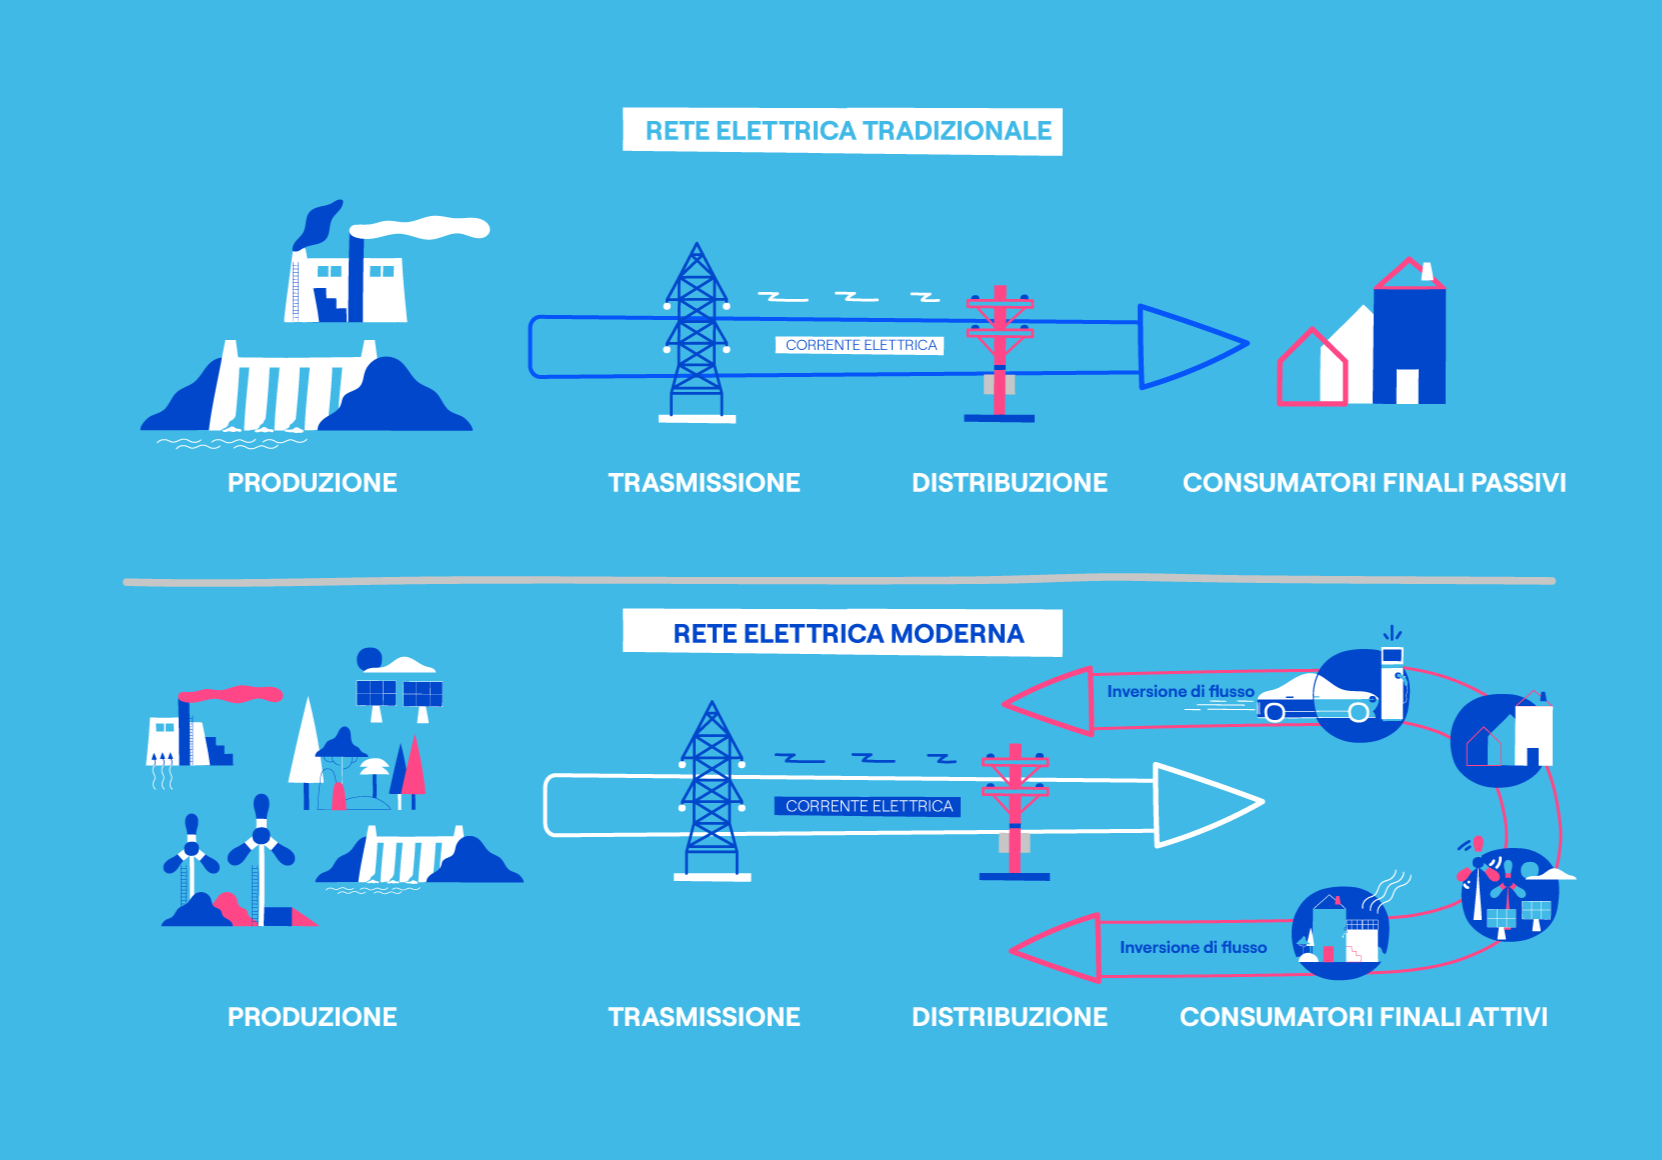
\includegraphics[width=0.8\linewidth]{img/Smart-Grid-EDistribuzione2.png}
    \caption{Confronto rete tradizionale e rete intelligente}
    \label{fig:TraditionalGridVSSmartrGrid}
\end{figure}


Come si può vedere nella Figura \ref{fig:TraditionalGridVSSmartrGrid} la Smart Grid si compone di 4 parti fondamentali: la \textit{Produzione}, la 
\textit{Trasmissione}, la \textit{Distribuzione} e infine le \textit{Utenze}.

% \begin{center}
%     \textit{Produzione} - \textit{Trasmissione} - \textit{Distribuzione} - \textit{Utenze}
% \end{center}

\newpage
\subsection{Produzione}

\begin{figure}[t]
    \centering
    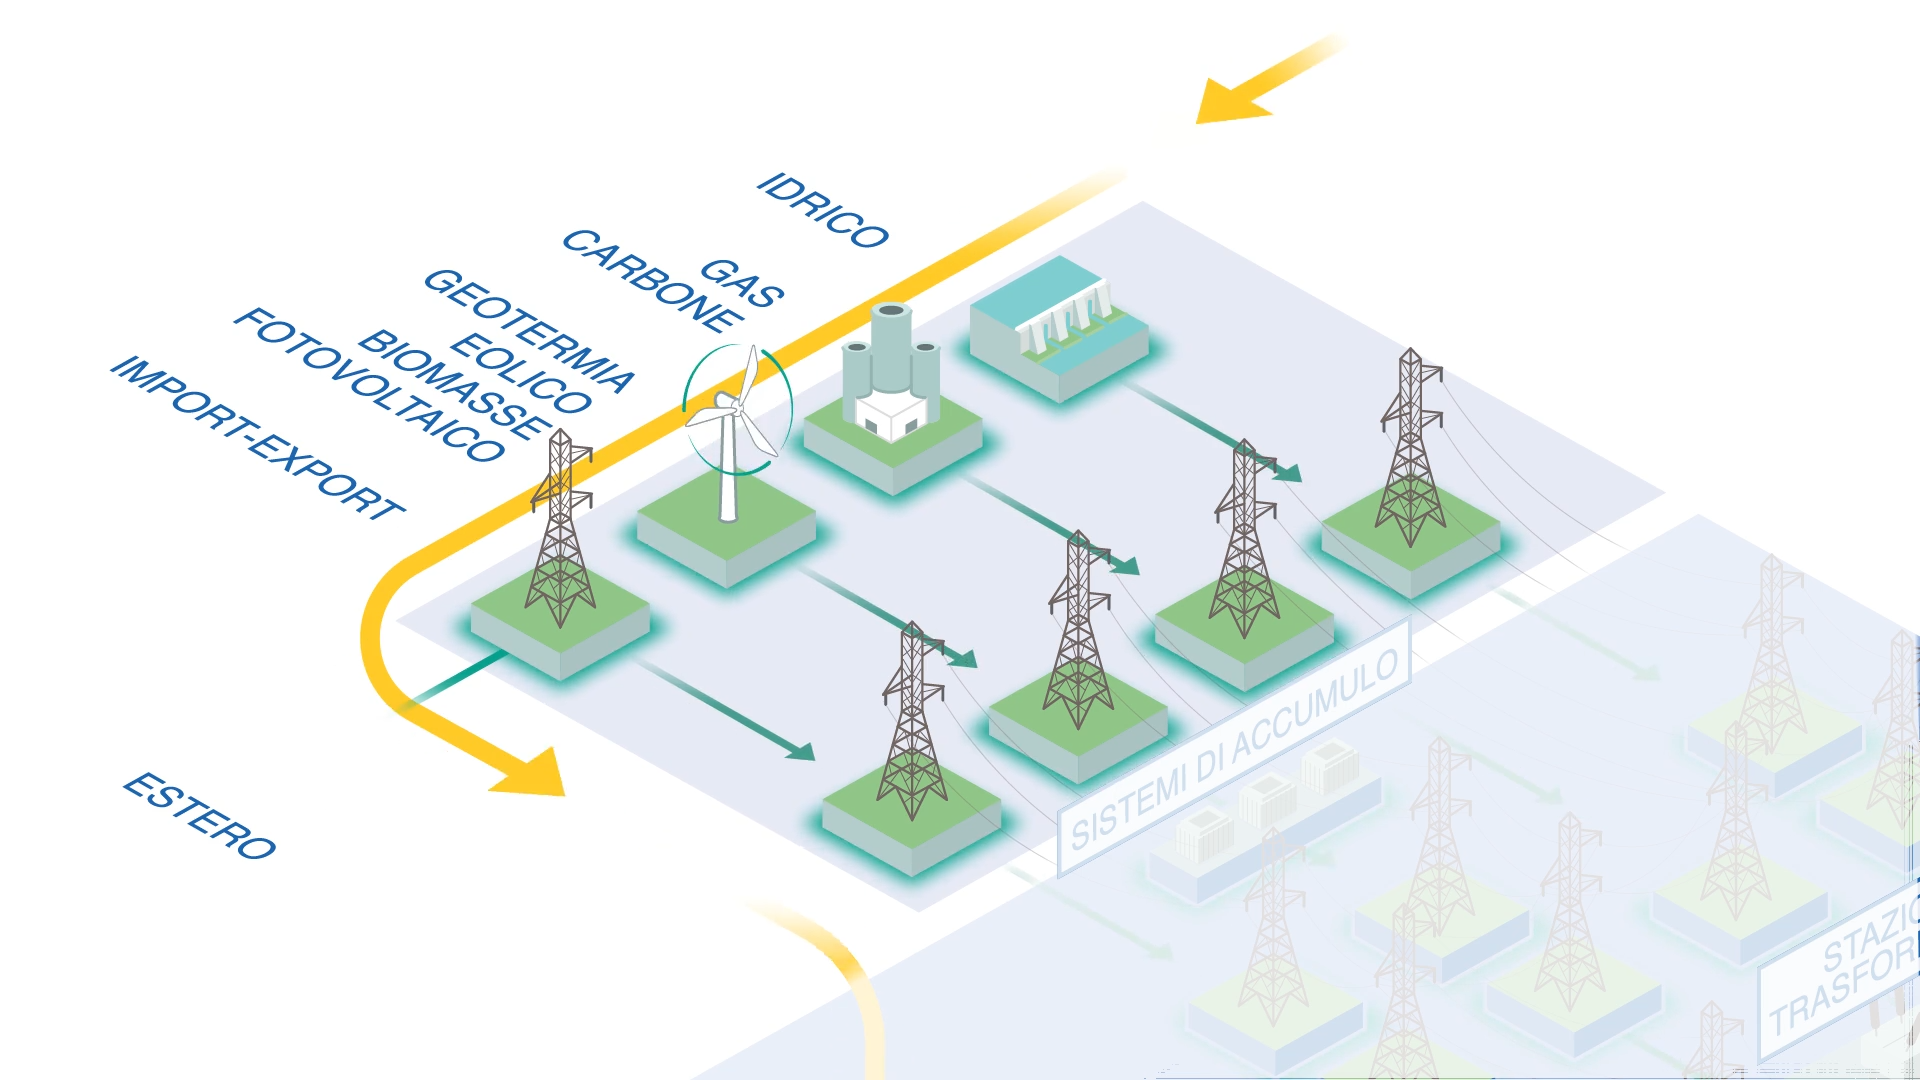
\includegraphics[width=0.9\linewidth]{img/Terna-Produzione.png}
    \caption{Produzione}
\end{figure}

La produzione di elettricità, sia nel sistema tradizionale sia con l'utilizzo delle Smart Grid, avviene attraverso un mix energetico di Fonti Energetiche non Rinnovabili (\textbf{non FER}) e Fonti Energetiche Rinnovabili (\textbf{FER}).

Il mix energetico italiano sfrutta varie fonti tra cui le non FER, con circa il 54\%, e il restante 46\% proviene invece dalle fonti FER Tabella \ref{tab:GSE-mix-nazionale-2023}.


\begin{table}[h!]
    \renewcommand{\arraystretch}{1.2}
    \centering
    \begin{tabular}{c|c}
        % \multicolumn{2}{c}{\shortstack{}}\\
         % \multicolumn{2}{c}{Fonti primarie utilizzate \%} \\
         Fonti primarie utilizzate	& \% \\
         \hline
         Fonti rinnovabili & 46 \\
         Gas naturale& 43 \\
         Carbone& 5 \\
         Altre fonti & 5 \\
         Prodotti petroliferi& 1 \\
    \end{tabular}
    \caption{Composizione del mix iniziale nazionale immessa nel anno 2023 \cite{GSE}}
    \label{tab:GSE-mix-nazionale-2023}
\end{table}



In particolare, come riportato nel "Rapporto Mensile sul Sistema Elettrico 2024" redatto da Terna \cite{TernaRapporto2024}, si mostra che l'assorbimento totale, la somma di produzione più importazioni di energia elettrica, nel periodo Gen-Dic 2024 è stata di $312\,TWh$, di cui FER \footnote{Produzione da FER = Idrico + Biomasse + Geotermico + Eolico + Fotovoltaico} $129\,TWh\,(49\,\%)$, non FER $132\,TWh\ (51\,\%)$ e importazioni $51\,TWh$ principalmente da Francia e Svizzera.

\newpage
\begin{figure}[h!]
    \centering
    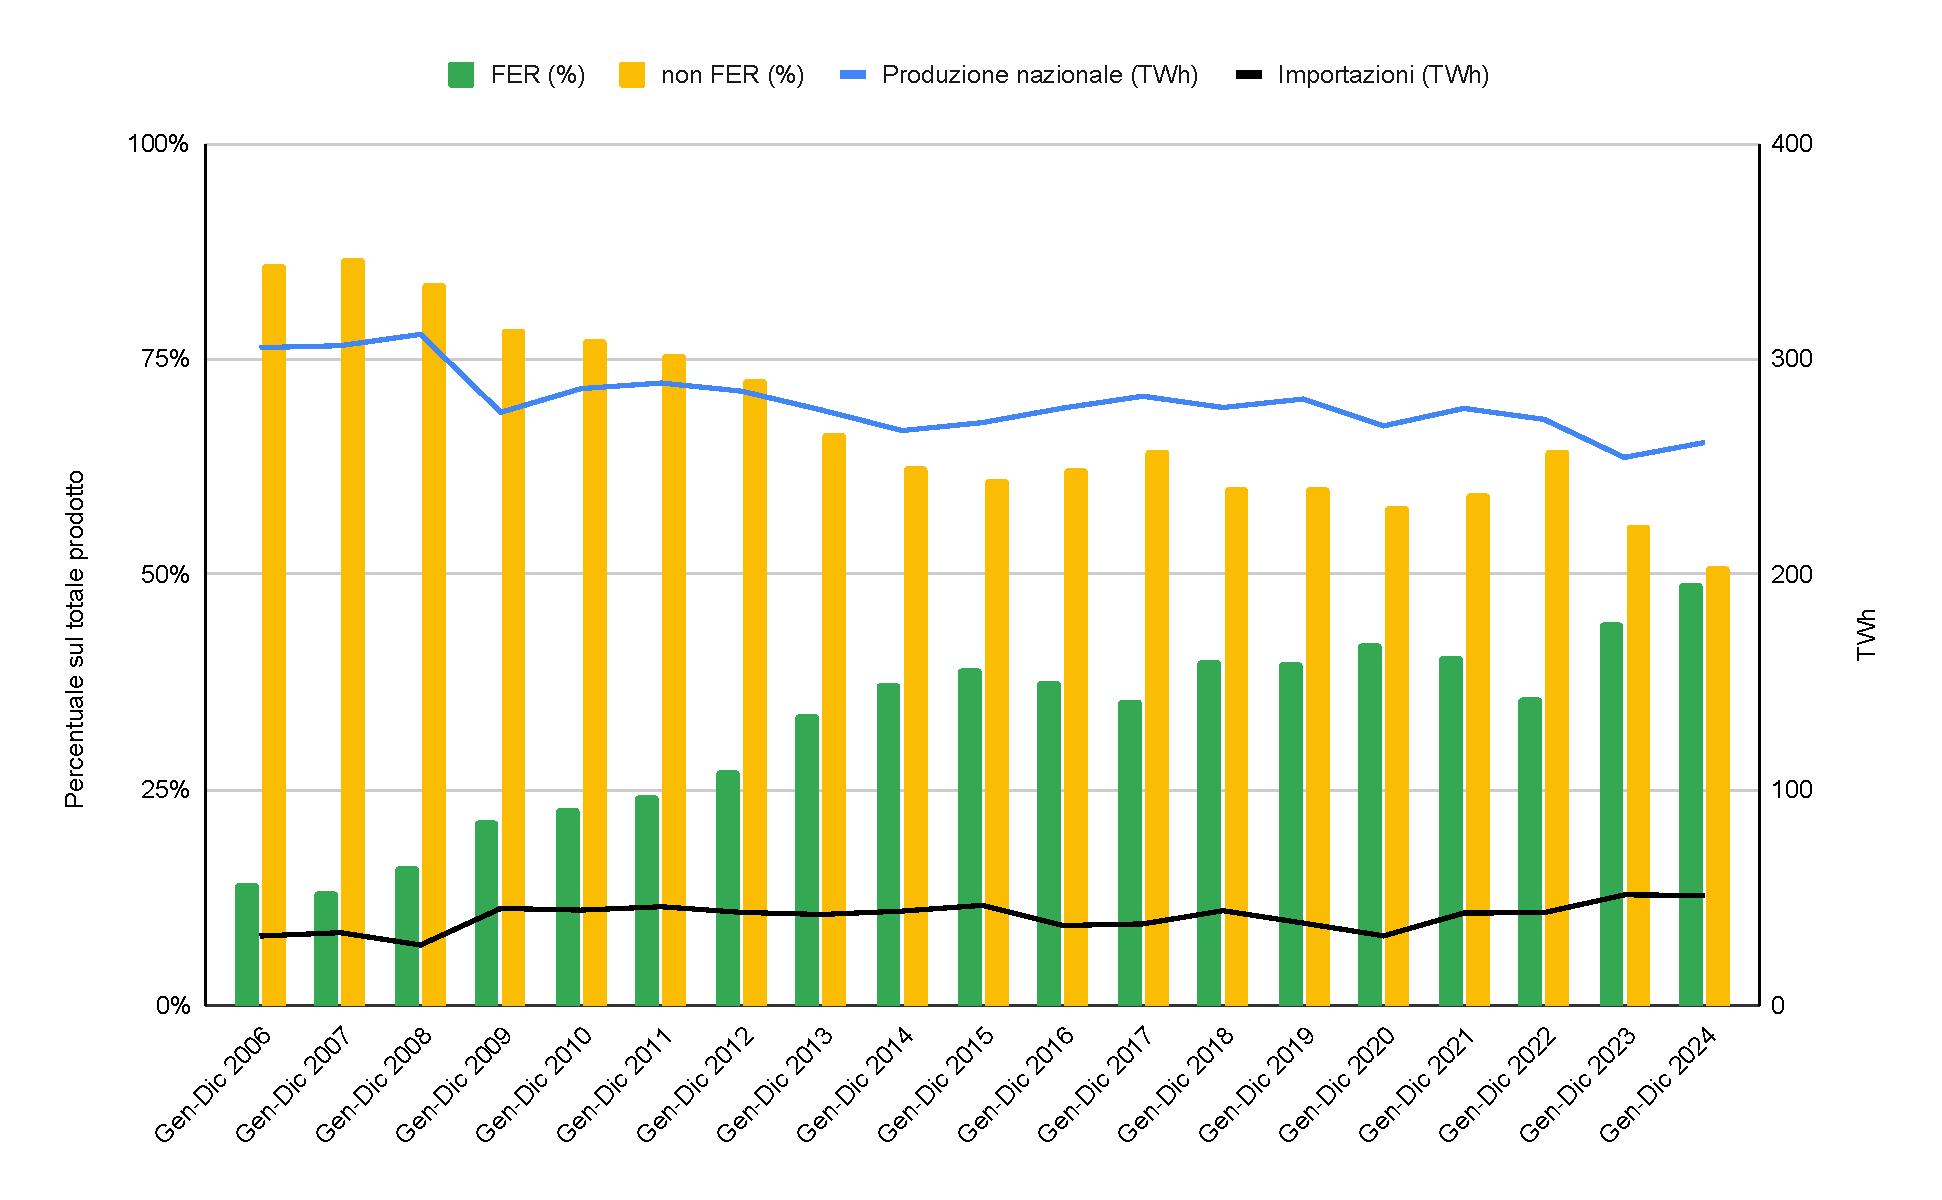
\includegraphics[trim= 1.1cm 0.95cm 1.15cm 1.05cm, clip, width=1\linewidth]{img/Terna-rapporto-annuale-2006-2024.pdf}
    \caption{Produzione nazionale annuale suddivisa tra FER e non FER \cite{terna-rapporto-mensile-sito}}
    \label{graph:Terna-rapporto-annuale-2006-2024}
\end{figure}

Si può vedere dal Grafico \ref{graph:Terna-rapporto-annuale-2006-2024} come dal 2006 al 2024 ci sia stato un incremento consistente della produzione di energia attraverso le fonti FER, arrivando quasi ad un break even nel 2024. In particolar modo, come si evince dal Grafico \ref{graph:Terna-FER-a-confronto-2006-2024}, questa crescita e stata possibile grazie all'installazione di pannelli fotovoltaici a partire dall'anno 2009 e il progressivo e costante aumento degli impani eolici.


\begin{figure}[h!]
    \centering
    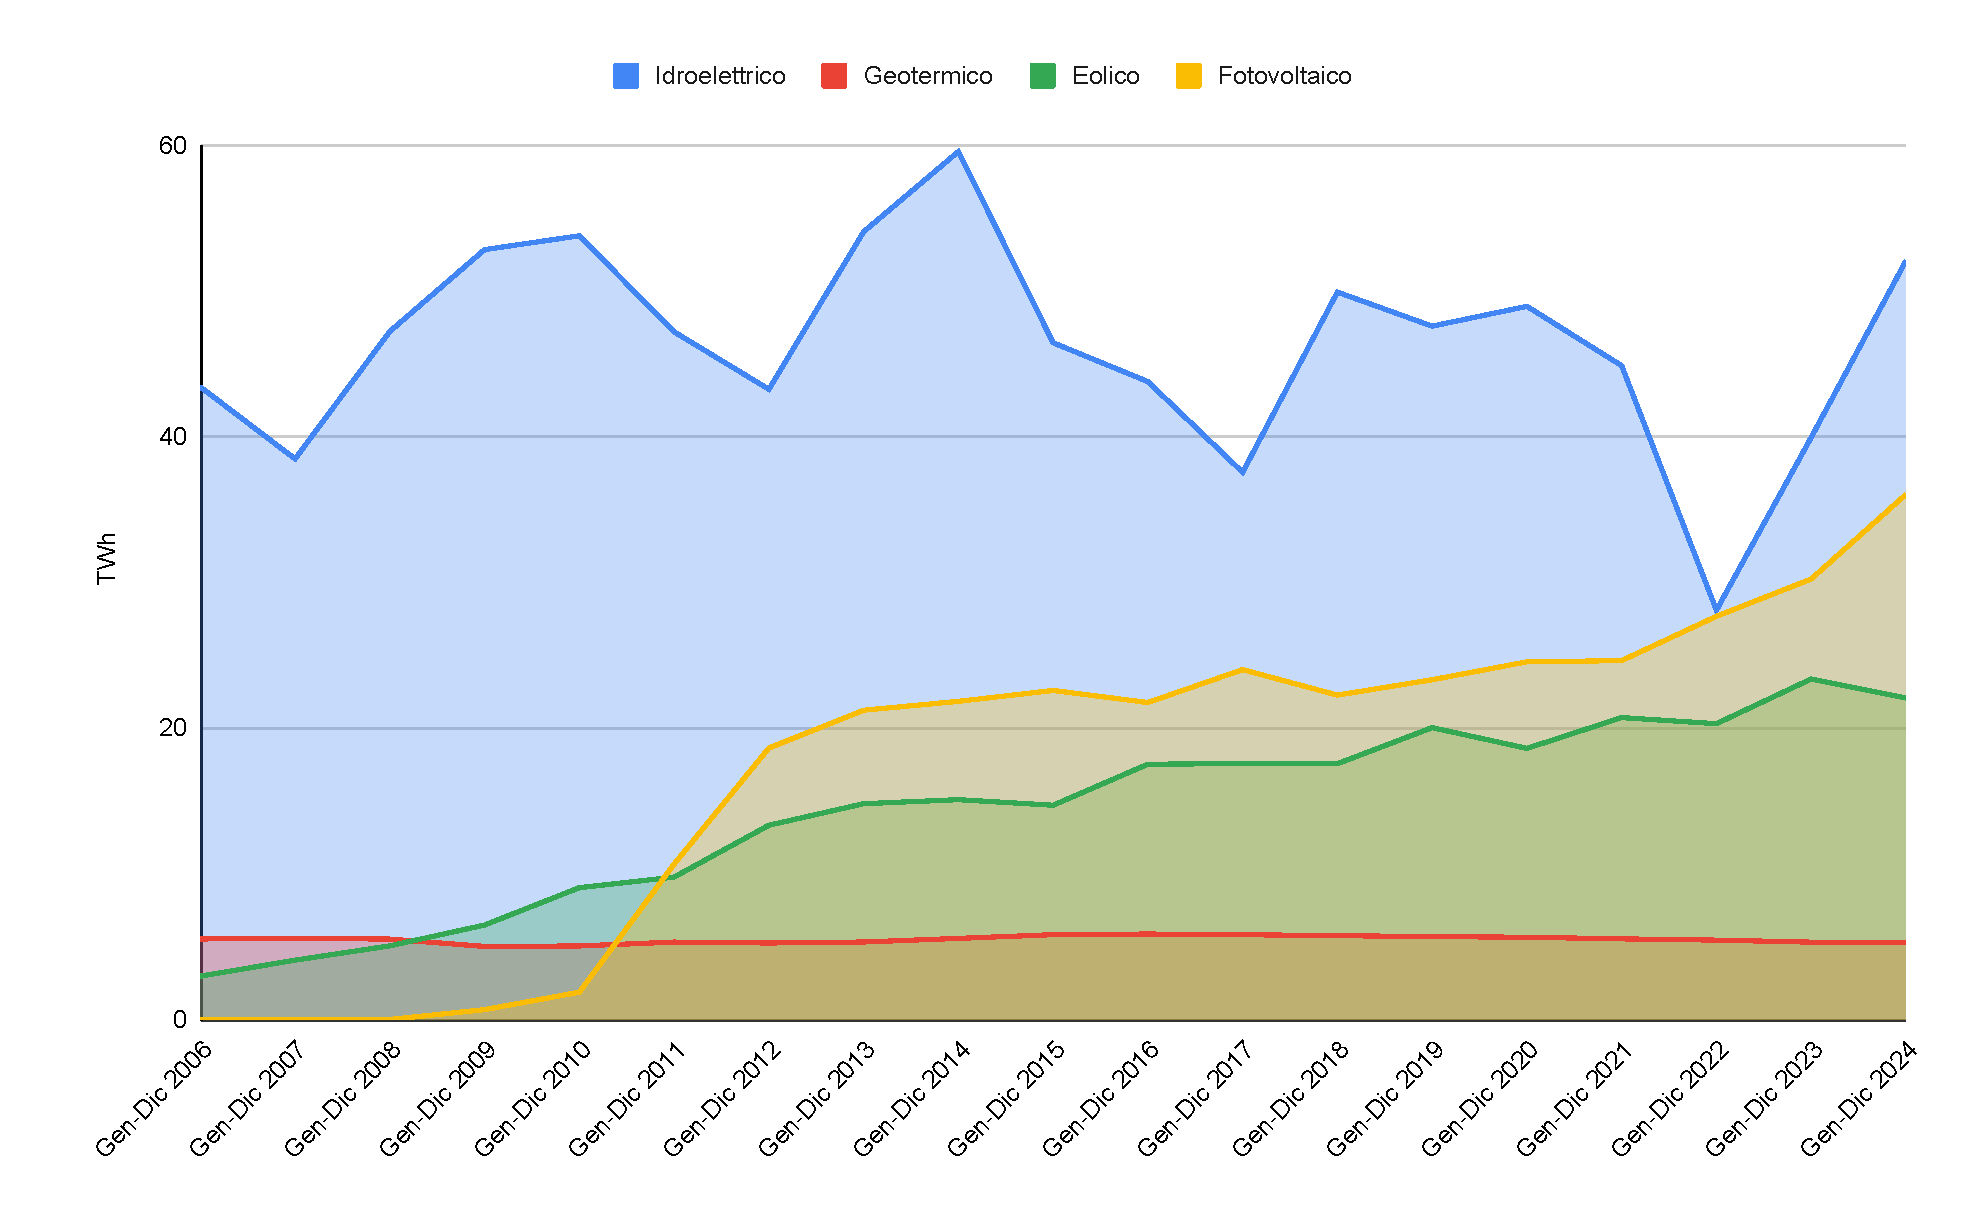
\includegraphics[trim= 1.6cm 1cm 0.85cm 1.05cm, clip, width=1\linewidth]{img/Terna-FER-a-confronto-2006-2024.pdf}
    \caption{Suddivisione delle principali FER in Italia \cite{terna-rapporto-mensile-sito}}
    \label{graph:Terna-FER-a-confronto-2006-2024}
\end{figure}


\subsection{Trasmissione}
La società italiana che, in un regime di monopolio naturale, si occupa della trasmissione e del dispacciamento è Terna. Questa modalità di governance è diffusa anche nel resto d'Europa, poiché è la configurazione ideale da mantenere per garantire una gestione, un mantenimento e uno sviluppo costante su tutta la Rete Elettrica Nazionale (RTN).

La trasmissione è un punto cruciale del dispacciamento dell'energia elettrica che comprende: 

\begin{itemize}
    \item il monitoraggio dei flussi energetici deviando l'energia nelle zone con più alto assorbimento
    \item le disposizioni per gestire l'esercizio coordinato di tutti gli elementi del sistema 
    \item la programmazione di riparazioni, l'allaccio di nuove linee e l'indisponibilità di pezzi della rete
    \item la previsione del fabbisogno energetico nazionale ora per ora
\end{itemize}

Tutto questo tenendo sempre in considerazione che la sinusoide di rete, dalla produzione all'utente finale viene impiegata una corrente alternata, in tutta Italia - ed Europa - deve, in qualsiasi istante, avere un oscillazione di $50\,Hz$, con tolleranza molto bassa nell'ordine di $\pm1\%$, e una tensione di $130\,V$.

\begin{figure}[h!]
    \centering
    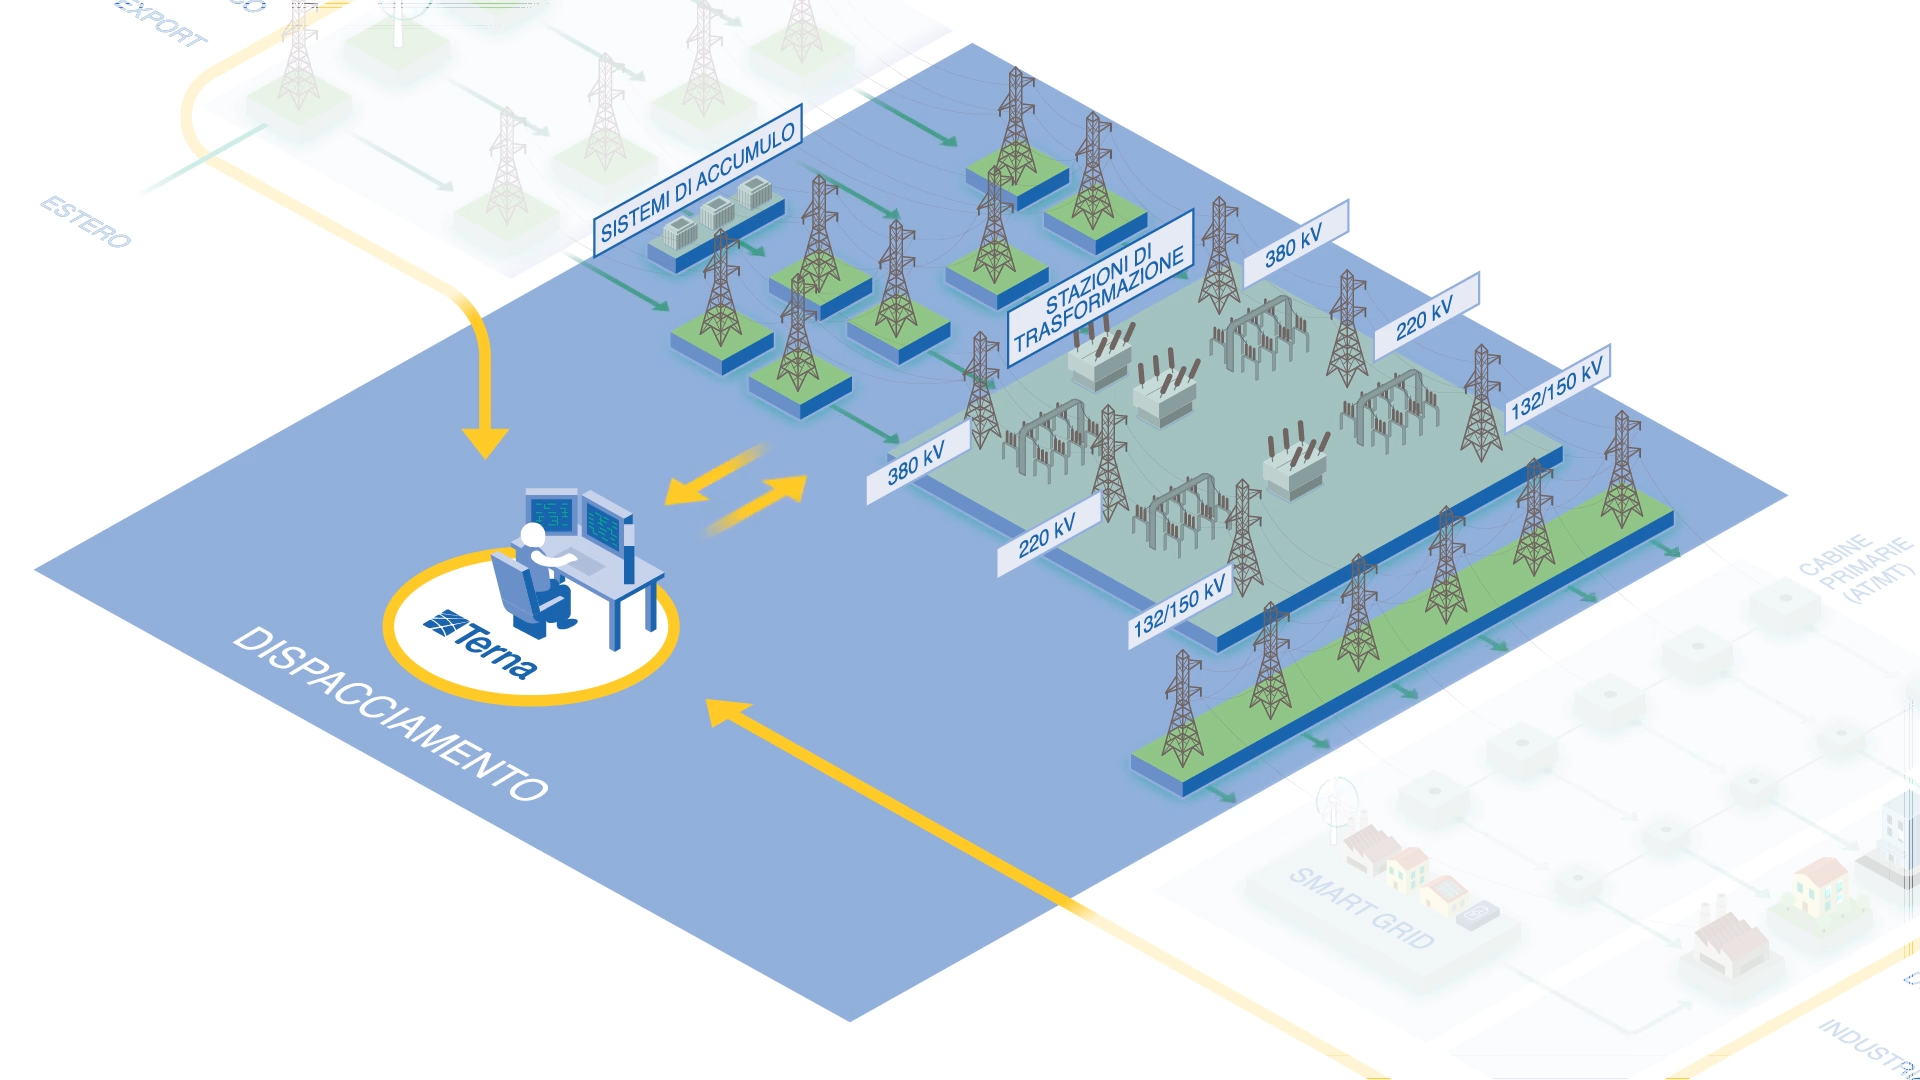
\includegraphics[width=0.9\linewidth]{img/Terna-Trasmissione.png}
    \caption{Trasmissione}
\end{figure}



\newpage
\subsection{Distribuzione}

In Italia, mentre per la trasmissione dell'elettricità, come detto in precedenza, è compito di Terna sulla base della concessione da parte dello Stato, la distribuzione dell'energia elettrica, è gestita da vari soggetti principalmente a livello territoriale.

Attualmente sul territorio nazionale sono $114$ le aziende \cite{arera-distributori} che operano nel settore della distribuzione dell'energia elettrica

Le principali, che servono assieme la quasi totalità dei cittadini dell'intero territorio nazionale sono:

\begin{itemize}
    
    \item E-Distribuzione: società del Gruppo Enel con ben 31.1 milioni di utenti serviti \cite{Clienti-sertivi-distribuzione} su tutto il territorio
    
    \item Areti: società del Gruppo Acea con 2,8 milioni di utenti operante nei territori di Roma e Formello \cite{Clienti-sertivi-areti}
    
    \item Unareti: società del Gruppo A2A con 1,2 milioni di utenti che gestisce i territori di Brescia, Milano e Bergamo \cite{Clienti-sertivi-uniareti}
    
    \item Ireti: società del Gruppo Iren con  700 mila utenti serviti nei territori di Parma, Torino e Vercelli \cite{Clienti-sertivi-ireti}
    
    \item Set Distribuzione: società del Gruppo Dolomiti Energia che serve il territorio della provincia autonoma di Trento con 330 mila utenze servite \cite{Clienti-sertivi-SetDistribuzione}
    
    \item V-reti: società del Gruppo AGSM AIM nata dall'integrazione tra Servizi a Rete (SAR) e Megareti. Sono 279 mila le utenze servite nel territorio di Verona e Vicenza  \cite{Clienti-sertivi-v-reti}
    
    \item Edyna: società del Gruppo Alperia, nata nel 2016 dalla fusione di Azienda EnergeticaReti e SELNET, distribuisce l'energia nel territorio altoatesino servendo 240 mila utenti.\cite{Clienti-sertivi-edyna}
    
    \item InRete: società del Gruppo Hera distribuisce l'energia a oltre 264 mila utenti in Emilia-Romagna e in Toscana  \cite{Clienti-sertivi-edyna}

    
\end{itemize}


Il distributore è responsabile del trasporto, della trasformazione e della consegna ad utenti finali e produttori dell'energia elettrica su reti in Media Tensione, da $1\,kV$ a $35\,kV$, e Bassa Tensione $<1kV$.
L'energia elettrica viene prelevata dalla rete ad Alta Tensione, da $35\,kV$ a $150\,kV$, e portata al livello di Media Tensione  all'interno delle Cabine Primarie.

\begin{figure}[h!]
    \centering
    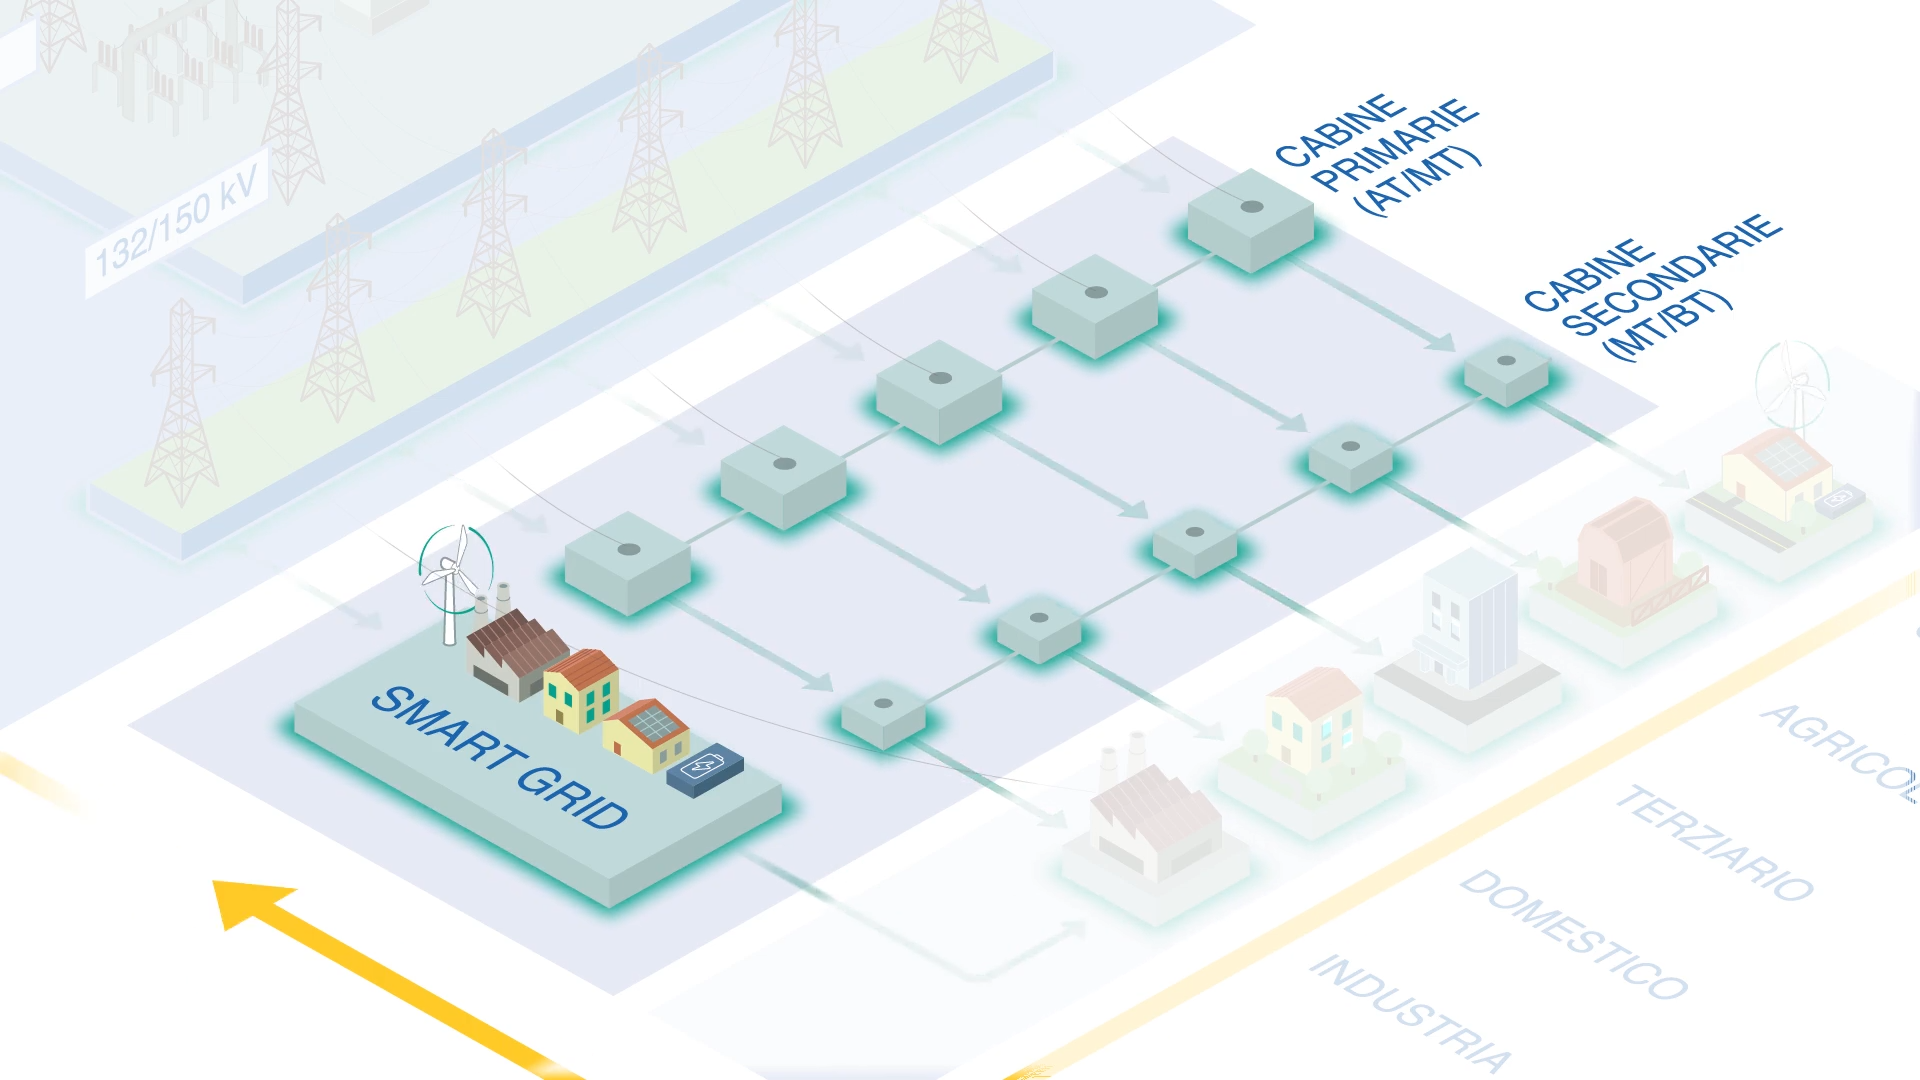
\includegraphics[width=0.9\linewidth]{img/Terna-Distribuzione.png}
    \caption{Distribuzione}
\end{figure}


\newpage
\subsection{Utenze finali}

\begin{figure}[h!]
    \centering
    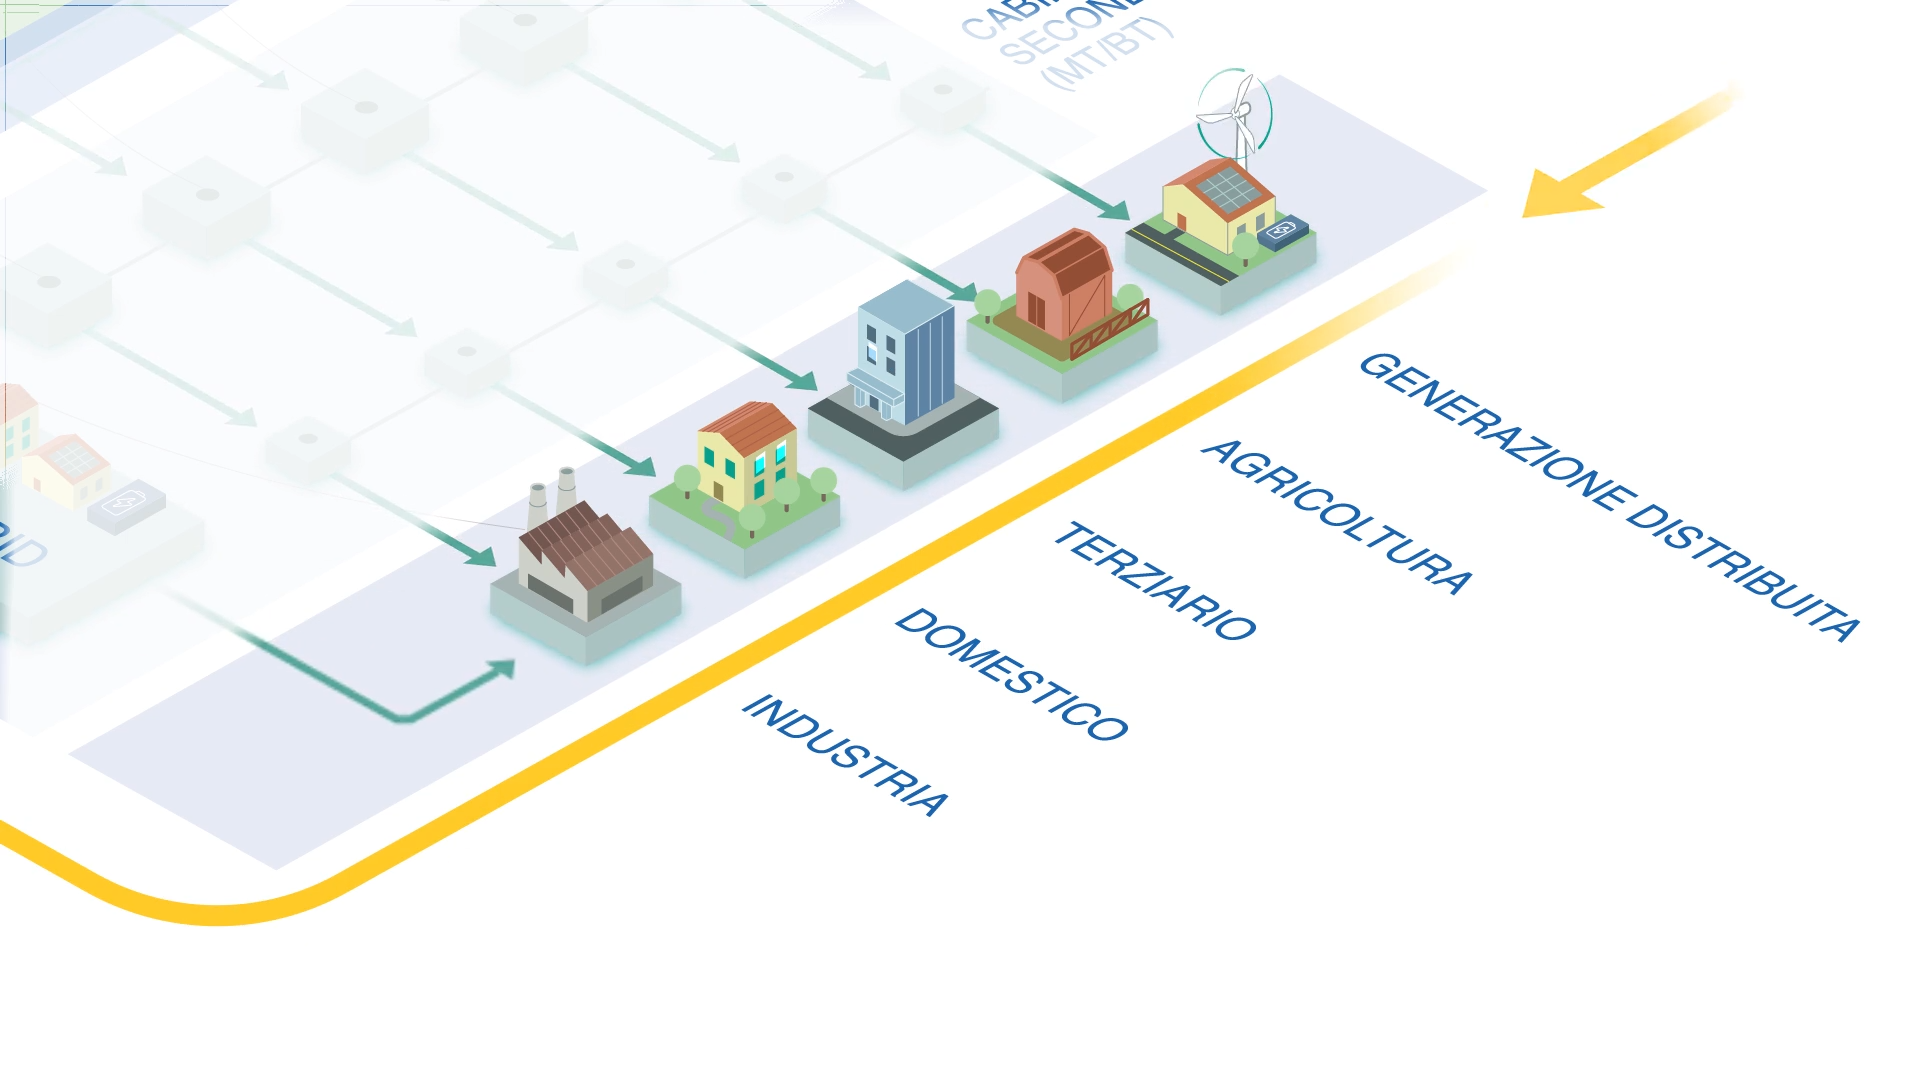
\includegraphics[width=0.9\linewidth]{img/Terna-Utenze.png}
    \caption{Utenze}
\end{figure}


Gli utenti finali possono scegliere il proprio venditore di energia elettrica in base alle specifiche esigenze e alle offerte di mercato.

Molto utile può essere infatti l'utilizzo de \href{https://www.ilportaleofferte.it/portaleOfferte/}{"Il portale delle offerte"} messo a disposizione proprio da ARERA. Questo comparatore fornisce all'utente finale una panoramica chiara di tutte le offerte disponibili sul mercato, questo per poter fare una scelta consapevole.


\section{Componenti principali della Smart Grid}

In questa sezione descriverò i domini relativi al consumatore e al livello più operazionale quale il dominio della trasmissione e distribuzione.

\subsection{Dominio del cliente}

Questo è il dominio più vicino al cliente ed è comporto da:

\begin{itemize}
    \item Smart Meter (\textbf{SM}) 
    \item Home/Building Energy Management Systems (\textbf{HEMS}/BEMS)
    \item Advanced Metering Infrastructure (\textbf{AMI})
\end{itemize}

\subsubsection{Smart Meter}

Gli Smart Meter, o più comunemente chiamati "contatori", sono quei dispositivi che ogni abitazione, negozio e azienda deve avere per allacciarsi alla rete elettrica.
Questo dispositivo conta quanti kWh (chilowattora) sono stati consumati da una specifica utenza e sulla basa di questo il venditore, con cui si ha stipulato il contratto, manderà la fattura da pagare.


Secondo il D. Lgs. 102/2014, che ha recepito la Direttiva Europea 2012/27/UE sull'efficienza energetica, tutti gli smart meter di prima generazione (1G) dovranno essere sostituiti con dei più moderni contatori di seconda generazione (2G) entro il 2035.

E-Distribuzione ha già completato questa transizione a fine del 2024 \cite{sostituzione-contatori-e-dist}, altri, come Ireti, prevedono di sostituirli completamente entro la fine del 2026 \cite{sostituzione-contatori-Ireti}.



